\section{Results}
\label{Results}

Forecasting this data was a definite challenge, and many of the more advanced statistical modeling methods would not adequately predict future data.  An initial approach to my time series forecasting efforts was using an Auto-Regressive Integrated Moving Average (ARIMA) model, but due to not having the decreasing trend present in the data, it performed very poorly.  After trying decomposition forecasting and receiving similar results, I resorted back to a basic polynomial regression.  I believe if I had more future data in the time series, those would have been better performing models.  Figure \ref{modelACC} illustrates the results given a 1 percent fatality rate. 



\begin{figure}[ht]
\centerline{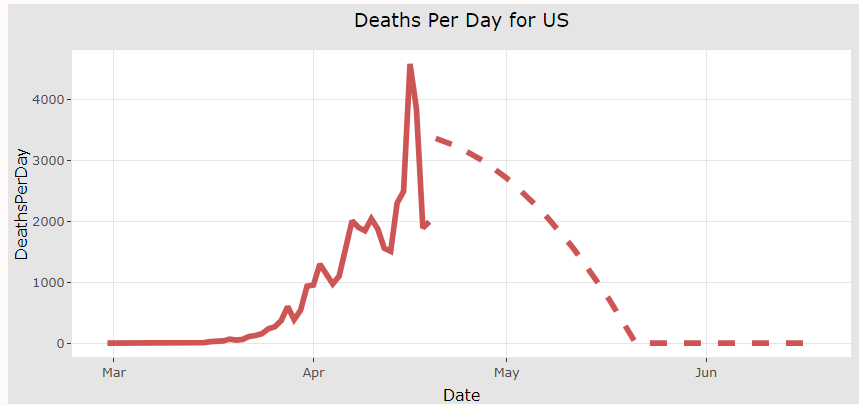
\includegraphics[scale=0.4]{Figures/Capture.PNG}}
\caption{Forecasting US Deaths Per Day}
\label{modelACC}
\end{figure}




While this quadratic rate of change is very simplistic and does not capture the full picture, it still gives an estimate of a hopeful decrease in daily fatalities.  The model predicts a drop to 0 daily deaths by early June.  This is likely not a realistic picture due to the plateauing nature observed in Italy and Spain. COVID-19 is an exponentially growing disease, so small differences in assumptions can make drastic effects on forecasts, and the data is not complete to illustrate the full picture.  Capturing R\typesubscript{0} over time as isolation and stay-at-home orders run their course is not an easy task.  

Another caveat of forecasting the fatality impact on the United States is the New York City metropolitan area's presence in the data.  This area was struck the hardest and the fastest with this pandemic, likely due to a massive and tightly congested population that relies so much on mass transit.  Many reports seem to suggest a decline in R\typesubscript{0} under 1, so cases are shrinking instead of growing.  While New York seems to be on the backside of this pandemic, many other regions are likely to increase in case load over the next several weeks, and the data is not convincing that the peak has been reached as a country.  This all depends on how open the public stays, and how effective social distancing can be in the United States compared to other countries with stricter guidelines. 

